\documentclass[tikz,border=2pt]{standalone}
\usepackage{amsmath,amssymb}
\usepackage{tikz}

\begin{document}
% Pascal's triangle: row n lists the binomial coefficients, the coefficients of (a+b)^n.
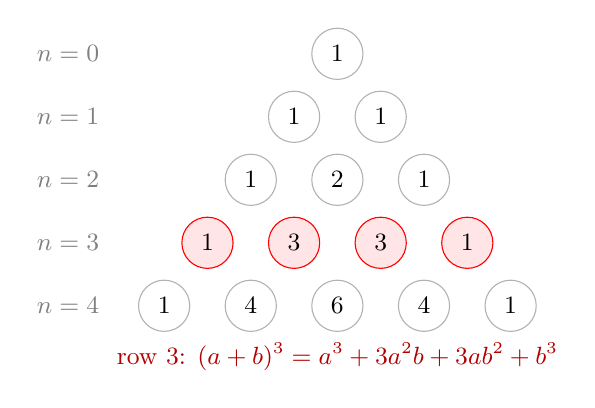
\begin{tikzpicture}[every node/.style={font=\small}]
	\foreach \n in {0,...,4} {
		\foreach \k in {0,...,\n} {
			\pgfmathtruncatemacro{\c}{round(factorial(\n)/(factorial(\k)*factorial(\n-\k)))}
			\ifnum\n=3
				\node[circle, draw=red, fill=red!10, inner sep=1pt, minimum size=6.5mm] at (\k*1.1-\n*0.55,-\n*0.8) {$\c$};
			\else
				\node[circle, draw=gray!60, inner sep=1pt, minimum size=6.5mm] at (\k*1.1-\n*0.55,-\n*0.8) {$\c$};
			\fi
		}
		\node[anchor=east, font=\small, gray] at (-2.9,-\n*0.8) {$n=\n$};
	}
	\node[red!70!black, anchor=north] at (0,-3.55) {row $3$: $(a+b)^3=a^3+3a^2b+3ab^2+b^3$};
	
\end{tikzpicture}
\end{document}
